\documentclass[a4paper]{article} %format de la feuille + type de document https://en.wikibooks.org/wiki/LaTeX/Document_Structure#Document_classes
%packages nécessaire pour nos besoins
\usepackage[utf8]{inputenc}
\usepackage[T1]{fontenc}
\usepackage[english,french]{babel}
\usepackage{amsmath}
\usepackage{amssymb,amsfonts,textcomp}
\usepackage{color}
\usepackage{array}
\usepackage{hhline}
\usepackage{hyperref}
\usepackage[pdftex]{graphicx}
\usepackage{sectsty}
\usepackage{tcolorbox}
\usepackage{textcomp}
\usepackage{courier}
\usepackage[font={small,it}]{caption}
\usepackage{float}
\usepackage{graphicx}
\usepackage{caption}
\usepackage{tabularx}
\usepackage{multirow}% http://ctan.org/pkg/multirow
\usepackage{tikz}
\usepackage[top=25mm,bottom=25mm,right=25mm,left=25mm]{geometry} 
\usepackage[export]{adjustbox}
\usepackage{listings}


%Définition des couleurs
\definecolor{havelockBlue}{rgb}{0.004, 0.42, 0.73}
\definecolor{Monokaimagenta}{rgb}{0.86,0.08,0.24}
\definecolor{codegray}{rgb}{0.5,0.5,0.5}
\definecolor{backcolour}{rgb}{0.95,0.95,0.92}

%utilisation de la couleur définie avant
%toutes les sections auront cette couleur
\sectionfont{\color{havelockBlue}}
%\subsectionfont{\color{havelockBlue}}
%début du document
\begin{document}

\renewcommand{\labelitemi}{$\bullet$}
\renewcommand{\labelitemii}{$\cdot$}
\renewcommand{\labelitemiii}{$\diamond$}
\renewcommand{\labelitemiv}{$\ast$}



\lstdefinelanguage[mips]{Assembler}{%
  % so listings can detect directives and register names
  alsoletter={.\$},
  % strings, characters, and comments
  morestring=[b]",
  morestring=[b]',
  morecomment=[l]\#,
  % instructions
  morekeywords={[1]abs,abs.d,abs.s,add,add.d,add.s,addi,addiu,addu,%
    and,andi,b,bc1f,bc1t,beq,beqz,bge,bgeu,bgez,bgezal,bgt,bgtu,%
    bgtz,ble,bleu,blez,blt,bltu,bltz,bltzal,bne,bnez,break,c.eq.d,%
    c.eq.s,c.le.d,c.le.s,c.lt.d,c.lt.s,ceil.w.d,ceil.w.s,clo,clz,%
    cvt.d.s,cvt.d.w,cvt.s.d,cvt.s.w,cvt.w.d,cvt.w.s,div,div.d,div.s,%
    divu,eret,floor.w.d,floor.w.s,j,jal,jalr,jr,l.d,l.s,la,lb,lbu,%
    ld,ldc1,lh,lhu,li,ll,lui,lw,lwc1,lwl,lwr,madd,maddu,mfc0,mfc1,%
    mfc1.d,mfhi,mflo,mov.d,mov.s,move,movf,movf.d,movf.s,movn,movn.d,%
    movn.s,movt,movt.d,movt.s,movz,movz.d,movz.s,msub,msubu,mtc0,mtc1,%
    mtc1.d,mthi,mtlo,mul,mul.d,mul.s,mulo,mulou,mult,multu,mulu,neg,%
    neg.d,neg.s,negu,nop,nor,not,or,ori,rem,remu,rol,ror,round.w.d,%
    round.w.s,s.d,s.s,sb,sc,sd,sdc1,seq,sge,sgeu,sgt,sgtu,sh,sle,%
    sleu,sll,sllv,slt,slti,sltiu,sltu,sne,sqrt.d,sqrt.s,sra,srav,srl,%
    srlv,sub,sub.d,sub.s,subi,subiu,subu,sw,swc1,swl,swr,syscall,teq,%
    teqi,tge,tgei,tgeiu,tgeu,tlt,tlti,tltiu,tltu,tne,tnei,trunc.w.d,%
    trunc.w.s,ulh,ulhu,ulw,ush,usw,xor,xori},
  % assembler directives
  morekeywords={[2].align,.ascii,.asciiz,.byte,.data,.double,.extern,%
    .float,.globl,.half,.kdata,.ktext,.set,.space,.text,.word},
  % register names
  morekeywords={[3]\$0,\$1,\$2,\$3,\$4,\$5,\$6,\$7,\$8,\$9,\$10,\$11,%
    \$12,\$13,\$14,\$15,\$16,\$17,\$18,\$19,\$20,\$21,\$22,\$23,\$24,%
    \$25,\$26,\$27,\$28,\$29,\$30,\$31,%
    \$zero,\$at,\$v0,\$v1,\$a0,\$a1,\$a2,\$a3,\$t0,\$t1,\$t2,\$t3,\$t4,
    \$t5,\$t6,\$t7,\$s0,\$s1,\$s2,\$s3,\$s4,\$s5,\$s6,\$s7,\$t8,\$t9,%
    \$k0,\$k1,\$gp,\$sp,\$fp,\$ra},
literate=
  {á}{{\'a}}1 {é}{{\'e}}1 {í}{{\'i}}1 {ó}{{\'o}}1 {ú}{{\'u}}1
  {Á}{{\'A}}1 {É}{{\'E}}1 {Í}{{\'I}}1 {Ó}{{\'O}}1 {Ú}{{\'U}}1
  {à}{{\`a}}1 {è}{{\`e}}1 {ì}{{\`i}}1 {ò}{{\`o}}1 {ù}{{\`u}}1
  {À}{{\`A}}1 {È}{{\'E}}1 {Ì}{{\`I}}1 {Ò}{{\`O}}1 {Ù}{{\`U}}1
  {ä}{{\"a}}1 {ë}{{\"e}}1 {ï}{{\"i}}1 {ö}{{\"o}}1 {ü}{{\"u}}1
  {Ä}{{\"A}}1 {Ë}{{\"E}}1 {Ï}{{\"I}}1 {Ö}{{\"O}}1 {Ü}{{\"U}}1
  {â}{{\^a}}1 {ê}{{\^e}}1 {î}{{\^i}}1 {ô}{{\^o}}1 {û}{{\^u}}1
  {Â}{{\^A}}1 {Ê}{{\^E}}1 {Î}{{\^I}}1 {Ô}{{\^O}}1 {Û}{{\^U}}1
  {œ}{{\oe}}1 {Œ}{{\OE}}1 {æ}{{\ae}}1 {Æ}{{\AE}}1 {ß}{{\ss}}1
  {ű}{{\H{u}}}1 {Ű}{{\H{U}}}1 {ő}{{\H{o}}}1 {Ő}{{\H{O}}}1
  {ç}{{\c c}}1 {Ç}{{\c C}}1 {ø}{{\o}}1 {å}{{\r a}}1 {Å}{{\r A}}1
  {€}{{\euro}}1 {£}{{\pounds}}1 {«}{{\guillemotleft}}1
  {»}{{\guillemotright}}1 {ñ}{{\~n}}1 {Ñ}{{\~N}}1 {¿}{{?`}}1
}[strings,comments,keywords]

\definecolor{CommentGreen}{rgb}{0,.6,0}
 \lstset{
   language=[mips]Assembler,
   backgroundcolor=\color{backcolour},   
   escapechar=@ \#, % include LaTeX code between `@' characters
   keepspaces,   % needed to preserve spacing with lstinline
   basicstyle=\footnotesize\ttfamily\bfseries,
   numberstyle=\footnotesize\ttfamily\bfseries,
   commentstyle=\color{CommentGreen},
   stringstyle=\color{cyan},
   showstringspaces=false,
   captionpos=b,
   numbers=left,
   keywordstyle=[1]\color{blue},    % instructions
   keywordstyle=[2]\color{magenta}, % directives
   keywordstyle=[3]\color{red},     % registers
 }    

\lstset{language=[mips]{Assembler}}
 

%début d'un titre
\begin{titlepage}
            %centre les éléments
	\centering
	
	{\scshape\LARGE \color{Monokaimagenta} Laboratoire \\  \par}
	
	%espace vertical de 1 mms
	\vspace{1cm}
	
	{\Large\itshape Sven Rouvinez \& Johanna Melly\par}
	
	%http://www.personal.ceu.hu/tex/spacebox.htm
	\vfill
	Professeur\par
	%met le texte en gras 
	\textbf{Carlos Andrés Pena} \par% ajoute une ligne 
	\vspace{1cm}
	Assistant\par
	\textbf{Gaëtan Matthey}
	
	\vfill

            %affiche la date actuelle
	{\large \today\par}
	
%fin de la page de titre
\end{titlepage}

\section{Objectifs du laboratoire}
Comprendre et démontrer la partie MEMORY ACCESS et le fonctionnement d'une pile en mémoire, ainsi qu'ajouter une instruction personnalisée.
\section{Étape 1}
\subsection{Point a}
Écrire un programme en assembleur qui effectue une écriture et une lecture de deux mots aux adresses 0x0004 et 0x0006.
\paragraph{Le fichier ci-dessous} écrit 2 mots aux adresses 0x0004 et 0x0006 et les lit.

\lstinputlisting[caption=main.S,label=et1a]{../labo4/mains/mainEt1a.S}

\begin{center}
\begin{tabular}{|c|c|c|c|c|}
    \hline
    LIGNE  & R0     & R1     & R2     & M[adr]\\
    \hline
    1      & 0x0012 &        &        &\\
    \hline
    2      & 0x0012 &        & 0x0034 &\\
    \hline
    3      & 0x0012 & 0x1200 & 0x0034 &\\
    \hline
    4      & 0x0012 & 0x1234 & 0x0034 &\\
    \hline
    6      & 0x0000 & 0x1234 & 0x0034 &\\
    \hline
    7      & 0x0000 & 0x1234 & 0x0034 & 0x1234\\
    \hline
    9      & 0x0056 & 0x1234 & 0x0034 &\\
    \hline
    10     & 0x0056 & 0x1234 & 0x0078 &\\
    \hline
    11     & 0x0056 & 0x5600 & 0x0078 &\\
    \hline
    12     & 0x0056 & 0x5678 & 0x0078 &\\
    \hline
    14     & 0x0004 & 0x5678 & 0x0078 &\\
    \hline
    15     & 0x0004 & 0x5678 & 0x5678 &\\
    \hline
    17     & 0x0004 & r3   & r1 & \\
    \hline
\end{tabular}
\end{center}


\paragraph{Les adresses des mémoires Mem\_High et Mem\_Low} valent 0x0008. Ceci vient de cette l'instruction de la ligne 6 du fichier main.S. Car nous travaillons en 16 bits donc les adresses seront multipliées par 2 au moment de leur traitement.
Pour cette étape, les valeurs 0x1234 et 0x5678 ont été utilisées pour être insérées dans les mémoires, respectivement aux adresses 0x0004 et 0x0006. Comme Mem\_low doit prendre les bits de poids faible, s'y trouveront les valeurs 0x34 et 0x78. Mem\_high, elle, doit prendre les bits de poids fort, ainsi y seront stockés 0x12 et 0x56.

\begin{figure}[H]
    \centering
    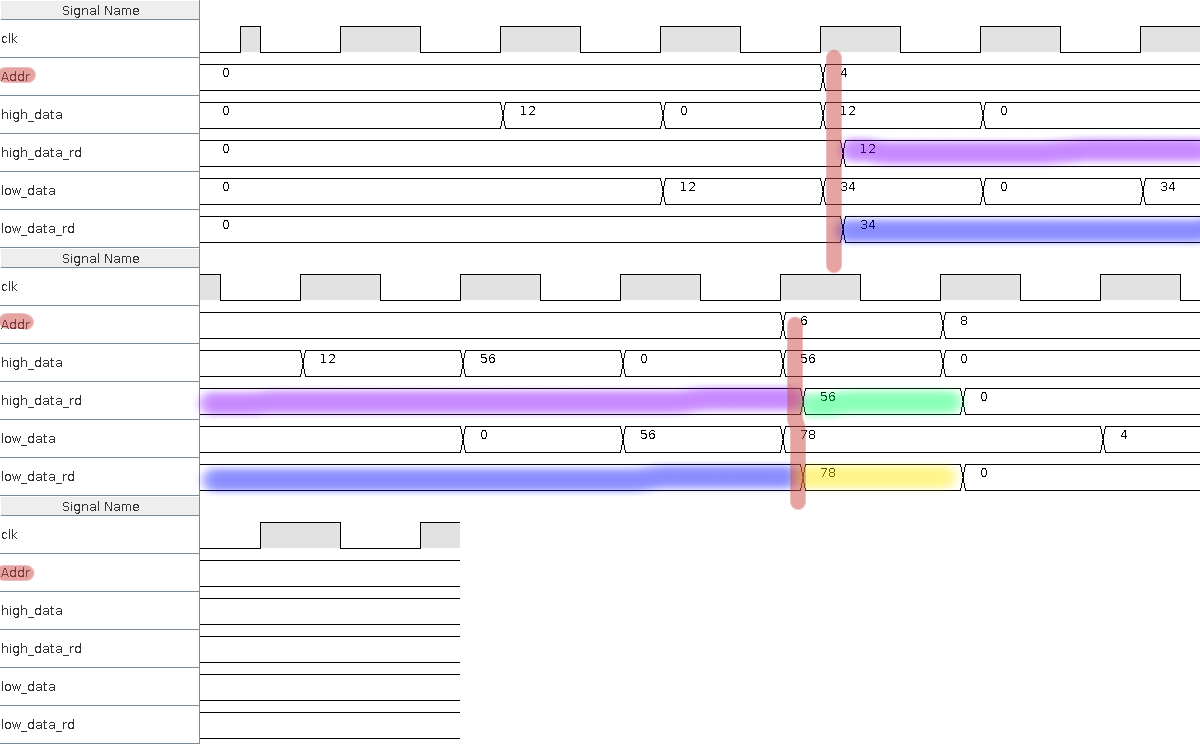
\includegraphics[width=1\textwidth]{src/CHRONO_ET1.png}
 \label{chrono_et1}
\end{figure}
Le chronogramme ci-dessus illustre le bon fonctionnement du programme assembleur. Les adresses mémoires sont en rouge. Les barres rouges signalent le passage à l'adresse 0x0004 et 0x0006. À la première barre rouge, les valeurs dans high\_data\_rg (violet) et low\_data\_rg (bleu) sont respectivement à 0x12 et à 0x34. À la deuxième barre rouge, les valeurs dans high\_data\_rg (vert) et low\_data\_rg (jaune)  sont respectivement à 0x56 et à 0x78.
\begin{figure}[H]
    \centering
    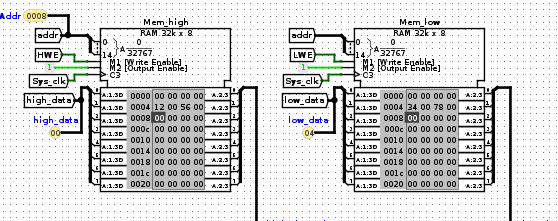
\includegraphics[width=.8\textwidth]{src/MEM_EXMPL.png}
    \captionof{figure}{Mémoires après écriture}
    \label{fig:mem_exmpl_pic}
\end{figure}

\subsection{Point b}
Effectuer une copie des deux mots écrits en point aux adresses 0x0014 et 0x0016 en utilisant uniquement les instructions LDRB et STRB.
\lstinputlisting[caption=main.S,label=et1a]{../labo4/mains/mainEt1b.S}

\section{Étape 2}
\lstinputlisting[caption=main.S,label=et1a]{../labo4/mains/mainEt2.S}
\section{Étape 3}
Modifier le circuit du processeur selon plusieurs conditions

\end{document}